% MSc dissertation example file, February 2022
%
% Leave one of the documentclass lines uncommented to match your degree.
% You may remove the logo option if it causes problems.
% Do not change any other options.
% \documentclass[logo,msc,adi]{infthesis}     % Adv Design Inf
% \documentclass[logo,msc,ai]{infthesis}      % AI
% \documentclass[logo,msc,cogsci]{infthesis}  % Cognitive Sci
% \documentclass[logo,msc,cs]{infthesis}      % Computer Sci
% \documentclass[logo,msc,cyber]{infthesis}   % Cyber Sec
% \documentclass[logo,msc,datasci]{infthesis} % Data Sci
% \documentclass[logo,msc,di]{infthesis}      % Design Inf
% \documentclass[logo,msc,dsti]{infthesis}    % Data Sci TI
% \documentclass[logo,msc,inf]{infthesis}     % Informatics
\documentclass[logo,msc]{infthesis}           % degree unspecified, do not change except to add your degree
%%%%%%%%%%%%%%%%%%%%%%%%
% Understand any problems and seek approval before assuming it's ok to remove ugcheck.
\usepackage{msccheck}

% Include any packages you need below, but don't include any that change the page
% layout or style of the dissertation. By including the ugcheck package above,
% you should catch most accidental changes of page layout though.

\usepackage{microtype} % recommended, but you can remove if it causes problems
\usepackage{caption}
\usepackage{subcaption}
\usepackage{url}
\usepackage{graphicx}
\usepackage{xcolor}
\usepackage{gnuplottex}
\usepackage{tikz}
\usetikzlibrary{arrows}
\usepackage{svg}

\begin{document}
\begin{preliminary}

\title{OpenTTDLab: A framework for repeatable, Replicable, \& Reproducible experiments using OpenTTD}

\author{Michal Charemza}

\date{\today}

\abstract{
OpenTTD is an open source business simulation game based on the 1994 game Transport Tycoon Deluxe, and in spite of being designed for recreation, OpenTTD has been used in a number of academic studies. However, these studies have problems regarding the repeatability, replicability, \& reproducibility of their experiments. In this dissertation, I present OpenTTDLab, a framework I created that allows OpenTTD to be used in a way that avoids these problems. I then show proof-of-concept results using this framework that I argue are repeatable, replicable, and reproducible; thus, giving evidence that OpenTTDLab can be a useful tool in future research.
}

\maketitle

\newenvironment{ethics}
   {\begin{frontenv}{Research Ethics Approval}{\LARGE}}
   {\end{frontenv}\newpage}

\begin{ethics}
This project was planned in accordance with the Informatics Research
Ethics policy. It did not involve any aspects that required approval
from the Informatics Research Ethics committee.

\standarddeclaration
\end{ethics}


\begin{acknowledgements}

Firstly thank you to Chris Sawyer, the original author of Transport Tycoon Deluxe: without you this project would not have existed. Then of course thank you to all the contributors of OpenTTLab over its 20 year history. And of these, thank you especially to Patric Stout (A.K.A. Truebrain), who not only gave advice and what I interpreted to be light blessing to this project, but also wrote the OpenTTD save game parser that OpenTTDLab originally forked from.

Thank you also to Ian Earle (A.K.A BasicBeluga) who found an issue in the documentation of OpenTTDLab and submitted a fix for it. While this was a small change, I took it as evidence that what I was creating stood a chance of being useful, and pushed me to continue.

Thank you to my supervisor Michael Hermann. His ongoing advice throughout this project has been invaluable, and I think also pushed me to do as good a job as I can.

Of course thank you to my husband Matthew Beach, whose support and advice was extremely helpful, and I cannot imagine living without. And finally, thank you to our dog, Elliot: he's a good boy.

\end{acknowledgements}


\tableofcontents
\end{preliminary}


\chapter{Introduction}

OpenTTD \cite{openttd} is an open source real time strategy (RTS) simulation game based on the 1994 game Transport Tycoon Deluxe by Chris Sawyer. The aim of the game is to successfully run a business by constructing networks of roads, railways, airports and ports, along with their respective vehicles, trains, planes and ships, in order to transport people and goods in exchange for money. OpenTTD is played on a simulated landscape as can be seen in Figure \ref{fig:openttd}.

\begin{figure}[h]
\centering
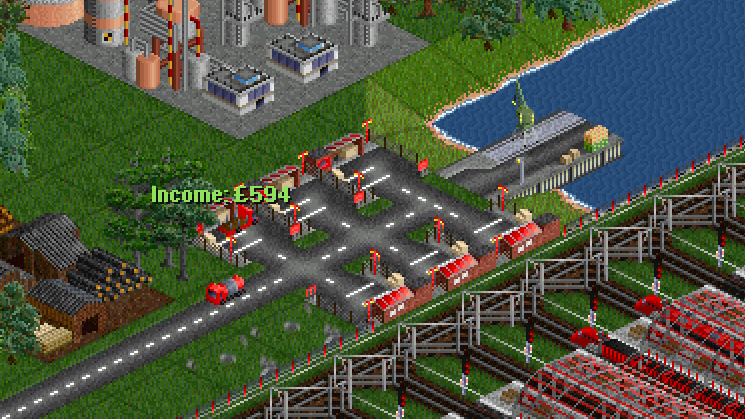
\includegraphics[width=\columnwidth]{assets/openttd-screenshot.png}
\caption{A small section of an OpenTTD (version 12.2) game at the moment when income is received for delivering goods by road. Also shown is part of a railway network, a port for ships, an oil refinery, and a sawmill.}
\label{fig:openttd}
\end{figure}


OpenTTD was created as a game for recreation. However, it is remarkably flexible: it has been successfully used as a tool to research artificial intelligence (AI) and machine learning (ML) algorithms \cite{wisniewski2011artificial, rios2009trains, bijlsma2014evolving}, scalability and mobile applications \cite{jiang2018mirroring}, and as a teaching aid \cite{HansenMuprhie2018}. It allows a single player to play in a non competitive world building mode, multiple human players playing cooperatively or competitively, and allows so-called custom AI-players that each control a company via code not part of the OpenTTD, but part of extensions to it written in the Squirrel language.

Using OpenTTD as a tool for research is the focus of this project, and specifically the focus is the development of a tool that augments its existing features for repeatable, replicable, \& reproducible research.

\section{A bit about the mechanics of the game?}

\section{A brief history of learning from simulation games}

Games have a long history of being used as tools beyond recreation, and specifically as tools to simulate the real world in order to take conclusions about the game environment and apply them to the world outside of the game, with war games doing this as far back even to ancient periods \cite{mayer2009gaming}. One of the world's oldest board game, Go (the `game of encircling territories' to literally translate its Mandarin name), originating in China approximately 4000 years ago and popular since, has been argued, to embody strategies that bear a striking resemblance to Chinese strategies of war and diplomacy, and these arguments have been paired with suggestions that Americans could better understand current (as of 2004) real-world Chinese strategies by learning Go \cite{lai2004learning}. Go is played on a grid, much like OpenTTD, suggesting also that OpenTTD's discretized simplification of space also has a long history in simulation.

The military-style/war games eventually evolved to logistic simulations, albeit still in military context. Fore example based MONOPOLOGS \cite{jackson1959learning} that is often credited as the first computerised logistics simulation game - SAY WHEN AND WHAT USED FOR. Then the MIT beer game - to illustrate something in supply chains. These then evolved to games that informed policy making - EXAMPLE.


This evolved [REF]

----

OpenTTD is part of a wider class of games: simulation games. Simulation games have been frequently used in various fields to explore scenarios in an effort to inform policies. PUT IN LIST.

Attention is usually paid to how realistic these games are. For example, \cite{raghothama2013review} summarises how well a number of games, including OpenTTD, how well the games model the real world. It's worth noting that while the economic model of OpenTTD is not realistic, \cite{raghothama2013review} classes some aspects of the transportation model as realistic, albeit without justification.



\section{Repeatability, Replicatability, \& Reproducibility}



The terms repeatability, replicability, and reproducibility unfortunately do not historically have universally agreed meanings \cite{plesser_reproducibility_2018}. To add to the confusion, the ACM have swapped their definitions reproducibility and replicability \cite{association_for_computing_machiner_new_2020}. For the avoidance of doubt, I use the ACM's definitions that are current as of October 2023 \cite{association_for_computing_machiner_artifact_2020}. For some results of an experiment conducted by a team of authors, where some computer-based artefacts were created to conduct these, these can be summarised as

\begin{description}
\item[Repeatability] The authors can obtain the results again, using the same artefacts.
\item[Reproducibility] A different team can obtain the results, using the original authors' artefacts.
\item[Replicability] A different team can obtain the results, without using any of the original authors' artefacts.
\end{description}

The strongest of these these, replicability, does not require a full re-implementation of all artifacts used in the research, but only those created by the original team. In OpenTTD terms, if an author writes a custom AI that is used in experiments, only that AI would need to be implemented by another team to replicate the research. OpenTTD itself would not need to be re-implemented in order for experiments to satisfy the definition of replicability.

Beyond just supplying definitions, the ACM also provide a system of 5 badges, as seen in Figure \ref{fig:acm_badges}. These can be applied to published research to incentivise research authors to make it so their research is reproducible and replicable by other teams. Other similar systems of badges are available.

\begin{figure}
     \centering
     \begin{subfigure}[t]{0.3\columnwidth}
         \centering
         
\includegraphics[width=\textwidth]{assets/artifacts_available.jpg}
         \caption{Artifacts available}
         \label{fig:y equals x}
     \end{subfigure}
     \hfill
     \begin{subfigure}[t]{0.3\columnwidth}
         \centering
         
\includegraphics[width=\textwidth]{assets/artifacts_evaluated_functional.jpg}
         \caption{Artifacts evaluated functional}
         \label{fig:three sin x}
     \end{subfigure}
     \hfill
     \begin{subfigure}[t]{0.3\columnwidth}
         \centering
         
\includegraphics[width=\textwidth]{assets/artifacts_evaluated_reusable.jpg}
         \caption{Artifacts evaluated reusable}
         \label{fig:five over x}
     \end{subfigure}
    \par\bigskip
     \begin{subfigure}[t]{0.3\columnwidth}
         \centering
         
\includegraphics[width=\textwidth]{assets/results_reproduced.jpg}
         \caption{Results reproduced}
         \label{fig:five over x}
     \end{subfigure}
     \begin{subfigure}[t]{0.3\columnwidth}
         \centering
         
\includegraphics[width=\textwidth]{assets/results_replicated.jpg}
         \caption{Results replicated  safd }
         \label{fig:five over x}
     \end{subfigure}
        \caption{The ACM system of badges for reproducble research}
        \label{fig:acm_badges}
\end{figure}

It is my hope that the framework presented here will make it more likely that research using OpenTTD will be not only repeatable, reproducible and replicable, but also more likely that upon publication, given all of these badges. 

\section{Review of research using OpenTTD}

\begin{itemize}
\begin{item}
Some papers list how they found all their upstream papers, in a light meta-analysis way. Worth it here? If I'm arguing something is lacking in particular, then maybe yes, because I sort of need evidence of an exhaustive search
\end{item}
\begin{item} Maybe this section could be split into using using OpenTTD in experiments, and just mentioning it
\end{item}
\begin{item}
\cite{fenjiro2018deep} - Mentions OpenTTD uses Deep Learning, but not partcular context or explanation. It doesn't really?? Do even any of the published AIs??
\end{item}
\end{itemize}

TODO: If we have the more structured / formal reproducibility stuff earlier, we can more properly judge the existing research.

From the found published research using OpenTTD, in my opinion there is yet to be a single case that couldn't offer significant improvements in at least one of its repeatability, replicability or replicability.

\subsection{Repeatability}

Repeatability should be the easiest of the 3Rs to achieve, especially with computer based simulation. However, much of the existing research using OpenTTD uses a low number of repeated experiments, with little or no statistical analysis, suggesting that it was not straightforward. The experiments of \cite{wisniewski2011artificial} were run just 3 times for example. The experiments in \cite{rios2009trains} were run 14 times, but not even for the same amount of in-game time.

\subsection{Reproducibility}

For reproducibility the author-supplied artifacts must be clear and available. There were references to modified OpenTTD in \cite{wisniewski2011artificial}, but the modified versions does not seem to be available. Potentially the authors could be contacted to supply their own artefacts, but this is not ideal, nor offers a strong guarantee that the artefacts supplied were exactly as they were that generated the results.

Also, the version of OpenTTD is not mentioned

The seeds of each experiements were also not supplied.

\subsection{Replicability}

This is the most difficult to judge without actually attempting to do it, and it is what.

However, if an experiemnt isn't even reproducible, it is even more difficult to replicate it.

\chapter{Existing features of OpenTTD}

\section{Review of OpenTTD command line options and configuration}
OpenTTD as of version 13.4 has over X command line options and Y configuration options that allow the player to customise how it behaves when playing. The ones that are particularly applicable to a  for repeatable, reproducible, and replicable research are reviewed below.

\subsection{Command line options}

\begin{description}
\item[-G \textless seed\textgreater] Allows the specification of the seed that initialises the random number generator that controls the pseudo random aspects of the game. For example, OpenTTD can auto generate landscapes. With the same seed (along with other configuration) one generation will be the same as the next
\item[-g] Starts a game immediately, rather than requiring the user to click through a introductory menu 
\item[-vnull:ticks=\textless number of ticks\textgreater] Puts the same into a "null" video mode that does not display the playing area on screen, and exits the game after a set number of \emph{ticks}. A tick is equal to approximately 1/Y of a day in game time.
\end{description}

The specification of the random seed should mean that OpenTTD affords exact repeatability and reproducibility when running as a simulation using only AI players. This means that it should be possible to make it straightfoward for to make results exactly reproducible, going beyond the requirements for ACM's badges on that front.

\subsection{Configuration options}

\begin{description}
\item[{fast\_forward\_speed\_limit} = \textless limit\textgreater] Limits the ticks per second the limit, which has a hard coded maximum in the game of 50000

\item[{[ai\_players]}] Allows the specification of which player are human and which are AI, and when they start playing.

\item[autosave = monthly|daily|other CHECK]

\item[keep\_all\_autosave]  A boolean value that allows all autosaves to be kept for further analysis
\end{description}


\section{The save game format}

OpenTTD saves its data in a custom binary format - its so-called savegame format. OpenTTD offers an extremely basic tool for extracting some data from this format. However, a separate Python based tool is available to extract data from save games

\section{What doesn't exist}

\begin{itemize}
\begin{item}
With reference to the the desired things from the reproducibility section, mention things that don't exist
\end{item}
\end{itemize}

\chapter{The framework}

The framework has two audiences. The first audience is an experimenter looking to conduct experiments with an AI, be it their own, or others, or a combination. The second is someone looking to reproduce or replicate another team's results. As such it contains separate instructions for both of these audiences.


\section{Design and creation process}

An agile process was used to design and create OpenTTDLab. The word agile has many meanings in developing software, but here I mean many iterations of lightweight design, coding, creating documentation and using what has been created. I often wrote light documentation of an API before coding it rather than after.

In this case this meant there were 3 sources of information that informed the design - the theoretical issues with existing with existing research with the features that the system should have to produce reproducible research of the previous chapter, writing documentation and imagining what it would be like to read and use, and my own practical experience using what has been written so far to either create tests of the framework, or create the results of the next chapter.

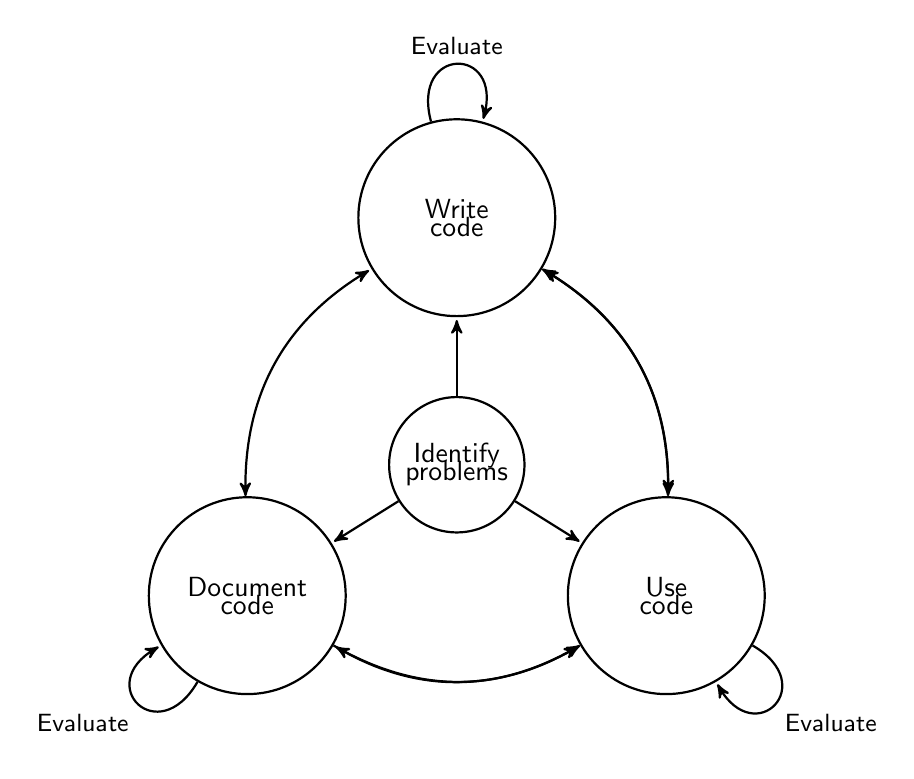
\begin{tikzpicture}[->,>=stealth',shorten >=1pt,auto,node distance=3cm,
                    thick,main node/.style={circle,draw,font=\sffamily}]

    % https://tex.stackexchange.com/a/102266
    \tikzset{
        position/.style args={#1:#2 from #3}{
            at=(#3.#1), anchor=#1+180, shift=(#1:#2)
        }
    }

    \node[main node, align=center] (reqs) {Identify\\[-2mm]problems};
    \node[main node, align=center,minimum size=2.5cm] (code) [position=90:1cm from reqs] {Write\\[-2mm]code};
    \node[main node, align=center,minimum size=2.5cm] (docs) [position=-148:1cm from reqs] {Document\\[-2mm]code};
    \node[main node, align=center,minimum size=2.5cm] (expe) [position=-32:1cm from reqs] {Use\\[-2mm]code};

    \path[every node/.style={font=\sffamily\small}]
        (reqs) edge [] node[] {} (code)
               edge [] node[] {} (expe)
               edge [] node[] {} (docs)
        (docs) edge [in=-150,out=-120,distance=1cm,loop] node {Evaluate} (docs)
               edge [bend left,arrows=<->] node[] {} (code)
               edge [bend right] node[left] {} (expe)
        (code) edge [distance=1cm,loop above] node {Evaluate} (code)
               edge [bend left,arrows=<->] node[] {} (expe)
        (expe) edge [in=-60,out=-30,distance=1cm,loop] node {Evaluate} (expe)
               edge [bend left,arrows=<->] node[] {} (docs)
               edge [bend right,arrows=<->] node[] {} (code);
\end{tikzpicture}

The first iterations were only based on documentation - no code existed. Later iterations were based on creating automated tests of the framework, and the final iterations were based mostly on my own experience using the code to find the results of the next chapter.

This process is based on Amazon's Working Backwards method, coupled with the Agile manifesto, and my own experience as a software and data engineer.

?? What about what open source software should have as well? Some of that in the introduction ??

Identify problems - always a choice of problems to solve. I think be extremely explicit in introduction on the problems! I think the whole repeatable, replicable and reproducible framework is a good list.

\section{Features}

\section{The experimenting team}

It takes the command line options in code, the various options of OpenTTD, and outputs two things:

\begin{itemize}
\item The results of the experiments - these are as Python variable, which allows the persistance of the results to be chosen by the experimenter. For example, in a basic CSV format.
\item The metadata of the experiments: the version of OpenTTD, the version of the framework itself, any commend line options, and all configuration, highlighting the configuration the differs from the defaults for that version of OpenTTD
\end{itemize}

\section{The reproducing or replicating team}

This leads to the second audience. The framework contains instructions to follow for a separate team trying to reproduce or replicate the experiments of the first team. These instructions mean that the first team can role-play as a reproducer or replicator, and test themselves how straightforward it is to reproduce the experiments, and judge for themselves if it is possible that their results be reproduced, and their research be awarded the badges of Figure \ref{fig:acm_badges}.

The replicability of results would be more difficult to judge - the author's artefacts cannot be used in this case, which means that if a team want to role play, they have to recreate their own artefacts, without reference to their original. The system here at least means that the "boilerplate" is handled, and this can be focused on.

\chapter{Example results from using the framework}

The framework has been used to extract how the bank balance from OpenTTD change over time for a company controlled by the TrainAI as in \label{fig:value-over-time}. The 

\begin{itemize}
  \item This has been created using a non-modified version of OpenTTD 13.1.
  \item The exact random seeds are shown
  \item There are 50 experiments run
  \item Each is run for the same amount of in game time
\end{itemize}

The output of the seeds used, all settings, OpenTTD version, without modification, should make the experiments repeatable, reproducible, and ideally replicable. Thus it is an improvement in these terms over many of the results reviewed in section 4.

A limitation of the framework is that the AI version used doesn't seem to have a version.

\begin{figure}[h]
\centering
\begin{gnuplot}[terminal=cairolatex,terminaloptions={size 5,3}]
set key autotitle columnhead
set datafile separator ","
set style fill pattern 2
set key left top
set key invert
set grid ytics
set format y "%.0s%c"
set xdata time
set format x "%Y"
set timefmt "%Y-%m-%d"
set xtics 3600*24*365
set mxtics 12
set ylabel 'Money in the bank $\textrm{\pounds}$'
set xlabel 'Date'
set xrange ["1950-01-01":"1953-02-01"]
plot 'assets/trainsai-means-standard-dev.csv' \ 
   every ::::36 using (timecolumn(1, '%Y-%m-%d')):($2+$3):($2-$3) with filledcurves lc rgb '#cccccc' title "$\\pm \\textrm{1 Standard deviation}$", \
   '' every ::::36 using (timecolumn(1, '%Y-%m-%d')):2 with lines title 'Mean', \
   '' every ::::36 using (timecolumn(1, '%Y-%m-%d')):($2+$3) with lines lc rgb '#cccccc' title '', \
   '' every ::::36 using (timecolumn(1, '%Y-%m-%d')):($2-$3) with lines lc rgb '#cccccc' title ''
\end{gnuplot}
\caption{The mean of money in the bank for TrainsAI over the first 36 months}
\label{fig:supplychainresiliance}
\end{figure}

\begin{figure}[h]
\centering
\begin{gnuplot}[terminal=cairolatex,terminaloptions={size 5,3}]
set key autotitle columnhead
set datafile separator ","
set style fill pattern 2
set key left top
set key invert
set grid ytics
set format y "%.0s%c"
set xtics 3600*24*365*5
set xdata time
set format x "%Y"
set timefmt "%Y-%m-%d"
set ylabel 'Money in the bank $\textrm{\pounds}$'
set xlabel 'Date'
set xrange ["1949-01-01":"1981-01-01"]
plot 'assets/trainsai-means-standard-dev.csv' \ 
   using (timecolumn(1, '%Y-%m-%d')):($2+$3):($2-$3) with filledcurves lc rgb '#cccccc' title "$\\pm \\textrm{1 Standard deviation}$", \
   '' using (timecolumn(1, '%Y-%m-%d')):2 with lines title 'Mean', \
   '' using (timecolumn(1, '%Y-%m-%d')):($2+$3) with lines lc rgb '#cccccc' title '', \
   '' using (timecolumn(1, '%Y-%m-%d')):($2-$3) with lines lc rgb '#cccccc' title ''
\end{gnuplot}
\caption{The mean of money in the bank for TrainsAI over time over 50 experiments for 30 years}
\label{fig:supplychainresiliance}
\end{figure}

\begin{figure}[h]
\centering
\begin{gnuplot}[terminal=cairolatex,terminaloptions={size 5,3}]
set key autotitle columnhead
set datafile separator ","
set style fill pattern 2
set key left top
set key invert
set grid ytics
set format y "%.0s%c"
set xdata time
set format x "%Y"
set timefmt "%Y-%m-%d"
set xtics 3600*24*365
set mxtics 12
set ylabel 'Money in the bank $\textrm{\pounds}$'
set xlabel 'Date'
set xrange ["1950-01-01":"1954-02-01"]
plot 'assets/pathzilla-means-standard-dev.csv' \ 
   every ::::48 using (timecolumn(1, '%Y-%m-%d')):($2+$3):($2-$3) with filledcurves lc rgb '#cccccc' title "$\\pm \\textrm{1 Standard deviation}$", \
   '' every ::::48 using (timecolumn(1, '%Y-%m-%d')):2 with lines title 'Mean', \
   '' every ::::48 using (timecolumn(1, '%Y-%m-%d')):($2+$3) with lines lc rgb '#cccccc' title '', \
   '' every ::::48 using (timecolumn(1, '%Y-%m-%d')):($2-$3) with lines lc rgb '#cccccc' title ''
\end{gnuplot}
\caption{The mean of money in the bank for Pathzilla over the first 48 months}
\label{fig:supplychainresiliance}
\end{figure}

\begin{figure}[h]
\centering
\begin{gnuplot}[terminal=cairolatex,terminaloptions={size 5,3}]
set key autotitle columnhead
set datafile separator ","
set style fill pattern 2
set key left top
set key invert
set grid ytics
set format y "%.0s%c"
set xtics 3600*24*365*5
set xdata time
set format x "%Y"
set timefmt "%Y-%m-%d"
set ylabel 'Money in the bank $\textrm{\pounds}$'
set xlabel 'Date'
set xrange ["1949-01-01":"1981-01-01"]
plot 'assets/pathzilla-means-standard-dev.csv' \ 
   using (timecolumn(1, '%Y-%m-%d')):($2+$3):($2-$3) with filledcurves lc rgb '#cccccc' title "$\\pm \\textrm{1 Standard deviation}$", \
   '' using (timecolumn(1, '%Y-%m-%d')):2 with lines title 'Mean', \
   '' using (timecolumn(1, '%Y-%m-%d')):($2+$3) with lines lc rgb '#cccccc' title '', \
   '' using (timecolumn(1, '%Y-%m-%d')):($2-$3) with lines lc rgb '#cccccc' title ''
\end{gnuplot}
\caption{The mean of money in the bank for Pathzilla over time over 50 experiments for 30 years}
\label{fig:supplychainresiliance}
\end{figure}


\begin{figure}[h]
\centering
\begin{gnuplot}[terminal=cairolatex,terminaloptions={size 5,3}]
set key autotitle columnhead
set datafile separator ","
set style fill pattern 2
set key left top
set key invert
set grid ytics
set format y "%.0s%c"
set xdata time
set format x "%Y"
set timefmt "%Y-%m-%d"
set xtics 3600*24*365
set mxtics 12
set ylabel 'Money in the bank $\textrm{\pounds}$'
set xlabel 'Date'
set xrange ["1950-01-01":"1954-02-01"]
plot 'assets/pathzilla-means-standard-dev.csv' \ 
   every ::::48 using (timecolumn(1, '%Y-%m-%d')):($2+$3):($2-$3) with filledcurves lc rgb '#cccccc' title "$\\pm \\textrm{1 Standard deviation}$", \
   '' every ::::48 using (timecolumn(1, '%Y-%m-%d')):2 with lines title 'Mean', \
   '' every ::::48 using (timecolumn(1, '%Y-%m-%d')):($2+$3) with lines lc rgb '#cccccc' title '', \
   '' every ::::48 using (timecolumn(1, '%Y-%m-%d')):($2-$3) with lines lc rgb '#cccccc' title '', \
    'assets/trainsai-means-standard-dev.csv' \ 
   every :::48 using (timecolumn(1, '%Y-%m-%d')):($2+$3):($2-$3) with filledcurves lc rgb '#cccccc' title "$\\pm \\textrm{1 Standard deviation}$", \
   '' every ::::48 using (timecolumn(1, '%Y-%m-%d')):2 with lines title 'Mean', \
   '' every ::::48 using (timecolumn(1, '%Y-%m-%d')):($2+$3) with lines lc rgb '#cccccc' title '', \
   '' every :::: using (timecolumn(1, '%Y-%m-%d')):($2-$3) with lines lc rgb '#cccccc' title ''
\end{gnuplot}
\caption{The mean of money in the bank for Pathzilla over the first 48 months}
\label{fig:supplychainresiliance}
\end{figure}

\begin{figure}[h]
\centering
\begin{gnuplot}[terminal=cairolatex,terminaloptions={size 5,3}]
set key autotitle columnhead
set datafile separator ","
set style fill pattern 2
set key left top
set key invert
set grid ytics
set format y "%.0s%c"
set xtics 3600*24*365*5
set xdata time
set format x "%Y"
set timefmt "%Y-%m-%d"
set ylabel 'Money in the bank $\textrm{\pounds}$'
set xlabel 'Date'
set xrange ["1949-01-01":"1981-01-01"]
plot 'assets/pathzilla-means-standard-dev.csv' \ 
   using (timecolumn(1, '%Y-%m-%d')):($2+$3):($2-$3) with filledcurves lc rgb '#cccccc' title "$\\pm \\textrm{1 Standard deviation}$", \
   '' using (timecolumn(1, '%Y-%m-%d')):2 with lines title 'Mean pathzilla', \
   '' using (timecolumn(1, '%Y-%m-%d')):($2+$3) with lines lc rgb '#cccccc' title '', \
   '' using (timecolumn(1, '%Y-%m-%d')):($2-$3) with lines lc rgb '#cccccc' title '', \
   'assets/trainsai-means-standard-dev.csv' \ 
   using (timecolumn(1, '%Y-%m-%d')):($2+$3):($2-$3) with filledcurves lc rgb '#cccccc' title "$\\pm \\textrm{1 Standard deviation}$", \
   '' using (timecolumn(1, '%Y-%m-%d')):2 with lines title 'Mean trainsai', \
   '' using (timecolumn(1, '%Y-%m-%d')):($2+$3) with lines lc rgb '#cccccc' title '', \
   '' using (timecolumn(1, '%Y-%m-%d')):($2-$3) with lines lc rgb '#cccccc' title ''
\end{gnuplot}
\caption{The mean of money in the bank for Pathzilla and TrainsAI over time over 50 experiments for 30 years}
\label{fig:supplychainresiliance}
\end{figure}

\begin{figure}[h]
\centering
\begin{gnuplot}[terminal=cairolatex,terminaloptions={size 5,3}]
set key autotitle columnhead
set datafile separator ","
set style fill pattern 2
set key left top
set key invert
set grid ytics
set format y "%.0s%c"
set xdata time
set format x "%Y"
set timefmt "%Y-%m-%d"
set xtics 3600*24*365
set mxtics 12
set ylabel 'Money in the bank $\textrm{\pounds}$'
set xlabel 'Date'
set xrange ["1950-01-01":"1954-02-01"]
plot 'assets/pathzilla-company-value-means-standard-dev.csv' \ 
   every ::::48 using (timecolumn(1, '%Y-%m-%d')):($2+$3):($2-$3) with filledcurves lc rgb '#cccccc' title "$\\pm \\textrm{1 Standard deviation}$", \
   '' every ::::48 using (timecolumn(1, '%Y-%m-%d')):2 with lines title 'Mean', \
   '' every ::::48 using (timecolumn(1, '%Y-%m-%d')):($2+$3) with lines lc rgb '#cccccc' title '', \
   '' every ::::48 using (timecolumn(1, '%Y-%m-%d')):($2-$3) with lines lc rgb '#cccccc' title ''
\end{gnuplot}
\caption{The mean of company value for Pathzilla over the first 48 months}
\label{fig:supplychainresiliance}
\end{figure}

\begin{figure}[h]
\centering
\begin{gnuplot}[terminal=cairolatex,terminaloptions={size 5,3}]
set key autotitle columnhead
set datafile separator ","
set style fill pattern 2
set key left top
set key invert
set grid ytics
set format y "%.0s%c"
set xtics 3600*24*365*5
set xdata time
set format x "%Y"
set timefmt "%Y-%m-%d"
set ylabel 'Money in the bank $\textrm{\pounds}$'
set xlabel 'Date'
set xrange ["1949-01-01":"1981-01-01"]
plot 'assets/pathzilla-company-value-means-standard-dev.csv' \ 
   using (timecolumn(1, '%Y-%m-%d')):($2+$3):($2-$3) with filledcurves lc rgb '#cccccc' title "$\\pm \\textrm{1 Standard deviation}$", \
   '' using (timecolumn(1, '%Y-%m-%d')):2 with lines title 'Mean', \
   '' using (timecolumn(1, '%Y-%m-%d')):($2+$3) with lines lc rgb '#cccccc' title '', \
   '' using (timecolumn(1, '%Y-%m-%d')):($2-$3) with lines lc rgb '#cccccc' title ''
\end{gnuplot}
\caption{The mean of company value for Pathzilla over time over 50 experiments for 30 years}
\label{fig:supplychainresiliance}
\end{figure}

\begin{figure}[h]
\centering
\begin{gnuplot}[terminal=cairolatex,terminaloptions={size 5,3}]
set datafile separator ","
set style fill pattern 2
set key left top
set key invert
set grid ytics
set format y "%.0s%c"
set xtics 3600*24*365*5
set xdata time
set format x "%Y"
set timefmt "%Y-%m-%d"
set ylabel 'Money in the bank $\textrm{\pounds}$'
set xlabel 'Date'
set xrange ["1949-01-01":"1961-01-01"]
plot 'assets/own-buses-means-standard_deviation.csv' \ 
   using (timecolumn(1, '%Y-%m-%d')):($2+$6):($2-$6) skip 2 with filledcurves lc rgb '#cccccc' title "$\\pm \\textrm{1 Standard deviation}$", \
   '' using (timecolumn(1, '%Y-%m-%d')):2 skip 2 with lines title 'Mean', \
   '' using (timecolumn(1, '%Y-%m-%d')):($2+$6) skip 2 with lines lc rgb '#cccccc' title '', \
   '' using (timecolumn(1, '%Y-%m-%d')):($2-$6) skip 2 with lines lc rgb '#cccccc' title ''
\end{gnuplot}
\caption{Money in the bank for my own simple AI: one bus}
\label{fig:supplychainresiliance}
\end{figure}

\begin{figure}[h]
\centering
\begin{gnuplot}[terminal=cairolatex,terminaloptions={size 5,3}]
set datafile separator ","
set style fill pattern 2
set key left top
set key invert
set grid ytics
set format y "%.0s%c"
set xtics 3600*24*365*5
set xdata time
set format x "%Y"
set timefmt "%Y-%m-%d"
set ylabel 'Money in the bank $\textrm{\pounds}$'
set xlabel 'Date'
set xrange ["1949-01-01":"1961-01-01"]
plot 'assets/own-buses-means-standard_deviation.csv' \ 
   using (timecolumn(1, '%Y-%m-%d')):($3+$7):($3-$7) skip 2 with filledcurves lc rgb '#cccccc' title "$\\pm \\textrm{1 Standard deviation}$", \
   '' using (timecolumn(1, '%Y-%m-%d')):3 skip 2 with lines title 'Mean', \
   '' using (timecolumn(1, '%Y-%m-%d')):($3+$7) skip 2 with lines lc rgb '#cccccc' title '', \
   '' using (timecolumn(1, '%Y-%m-%d')):($3-$7) skip 2 with lines lc rgb '#cccccc' title ''
\end{gnuplot}
\caption{Money in the bank for my own simple AI: two buses}
\label{fig:supplychainresiliance}
\end{figure}

\begin{figure}[h]
\centering
\begin{gnuplot}[terminal=cairolatex,terminaloptions={size 5,3}]
set datafile separator ","
set style fill pattern 2
set key left top
set key invert
set grid ytics
set format y "%.0s%c"
set xtics 3600*24*365*5
set xdata time
set format x "%Y"
set timefmt "%Y-%m-%d"
set ylabel 'Money in the bank $\textrm{\pounds}$'
set xlabel 'Date'
set xrange ["1949-01-01":"1961-01-01"]
plot 'assets/own-buses-means-standard_deviation.csv' \ 
   using (timecolumn(1, '%Y-%m-%d')):($4+$8):($4-$8) skip 2 with filledcurves lc rgb '#cccccc' title "$\\pm \\textrm{1 Standard deviation}$", \
   '' using (timecolumn(1, '%Y-%m-%d')):4 skip 2 with lines title 'Mean', \
   '' using (timecolumn(1, '%Y-%m-%d')):($4+$8) skip 2 with lines lc rgb '#cccccc' title '', \
   '' using (timecolumn(1, '%Y-%m-%d')):($4-$8) skip 2 with lines lc rgb '#cccccc' title ''
\end{gnuplot}
\caption{Money in the bank for my own simple AI: 4 buses}
\label{fig:supplychainresiliance}
\end{figure}

\begin{figure}[h]
\centering
\begin{gnuplot}[terminal=cairolatex,terminaloptions={size 5,3}]
set datafile separator ","
set style fill pattern 2
set key left top
set key invert
set grid ytics
set format y "%.0s%c"
set xtics 3600*24*365*5
set xdata time
set format x "%Y"
set timefmt "%Y-%m-%d"
set ylabel 'Money in the bank $\textrm{\pounds}$'
set xlabel 'Date'
set xrange ["1949-01-01":"2001-01-01"]
plot 'assets/own-buses-means-standard_deviation.csv' \ 
   using (timecolumn(1, '%Y-%m-%d')):6 skip 2 with lines title 'Mean 16 buses', \
   '' using (timecolumn(1, '%Y-%m-%d')):5 skip 2 with lines title 'Mean 8 buses', \
   '' using (timecolumn(1, '%Y-%m-%d')):4 skip 2 with lines title 'Mean 4 buses', \
   '' using (timecolumn(1, '%Y-%m-%d')):3 skip 2 with lines title 'Mean 2 buses', \
   '' using (timecolumn(1, '%Y-%m-%d')):2 skip 2 with lines title 'Mean 1 bus'
\end{gnuplot}
\caption{Money in the bank for my own simple AI: 1 vs 16 buses}
\label{fig:supplychainresiliance}
\end{figure}

\begin{figure}[h]
\centering
\begin{gnuplot}[terminal=cairolatex,terminaloptions={size 5,3}]
set datafile separator ","
set style fill pattern 2
set key left top
set key invert
set grid ytics
set format y "%.0s%c"
set xtics 3600*24*365*5
set xdata time
set format x "%Y"
set timefmt "%Y-%m-%d"
set ylabel 'Money in the bank $\textrm{\pounds}$'
set xlabel 'Date'
set xrange ["1949-01-01":"2001-01-01"]
plot 'assets/own-buses-means-standard_deviation.csv' \ 
   using (timecolumn(1, '%Y-%m-%d')):($6+$10):($6-$10) skip 2 with filledcurves lc rgb '#cccccc' title "$\\pm \\textrm{1 Standard deviation}$", \
   '' using (timecolumn(1, '%Y-%m-%d')):6 skip 2 with lines title 'Mean 16 buses', \
   '' using (timecolumn(1, '%Y-%m-%d')):($6+$10) skip 2 with lines lc rgb '#cccccc' title '', \
   '' using (timecolumn(1, '%Y-%m-%d')):($6-$10) skip 2 with lines lc rgb '#cccccc' title '', \
   '' using (timecolumn(1, '%Y-%m-%d')):($2+$6):($2-$6) skip 2 with filledcurves lc rgb '#cccccc' title "$\\pm \\textrm{1 Standard deviation}$", \
   '' using (timecolumn(1, '%Y-%m-%d')):2 skip 2 with lines title 'Mean 1 bus', \
   '' using (timecolumn(1, '%Y-%m-%d')):($2+$6) skip 2 with lines lc rgb '#cccccc' title '', \
   '' using (timecolumn(1, '%Y-%m-%d')):($2-$6) skip 2 with lines lc rgb '#cccccc' title ''
\end{gnuplot}
\caption{Money in the bank for my own simple AI: 1 vs 16 buses}
\label{fig:supplychainresiliance}
\end{figure}



\begin{figure}[h]
\centering
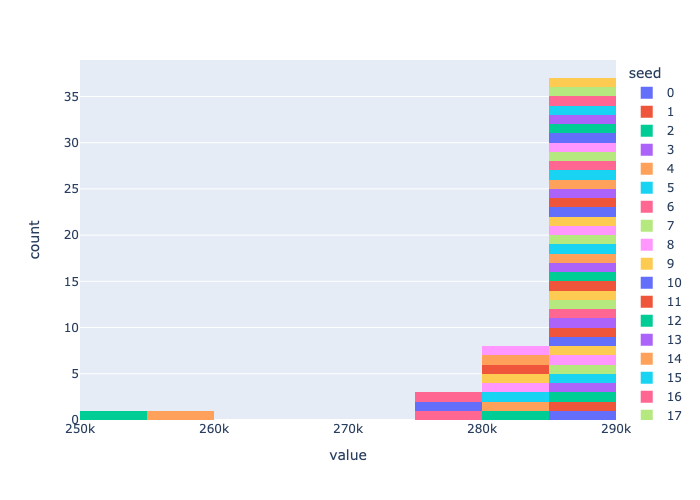
\includegraphics[width=\columnwidth]{assets/end-of-first-year-distribution.png}
\caption{A chart showing the balance over for 50 experiments (current OpenTTDLab )}
\label{fig:first-year}
\end{figure}

\begin{figure}[h]
\centering
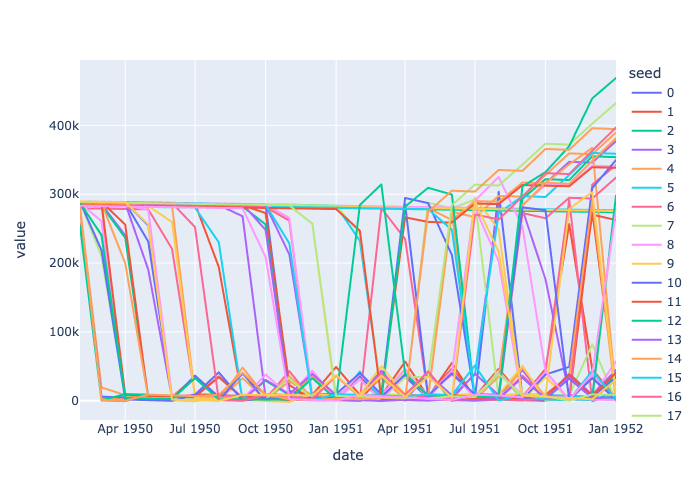
\includegraphics[width=\columnwidth]{assets/first-2-years.png}
\caption{A chart showing the balance over for 50 experiments (current OpenTTDLab )}
\label{fig:first-year}
\end{figure}

\begin{figure}[h]
\centering
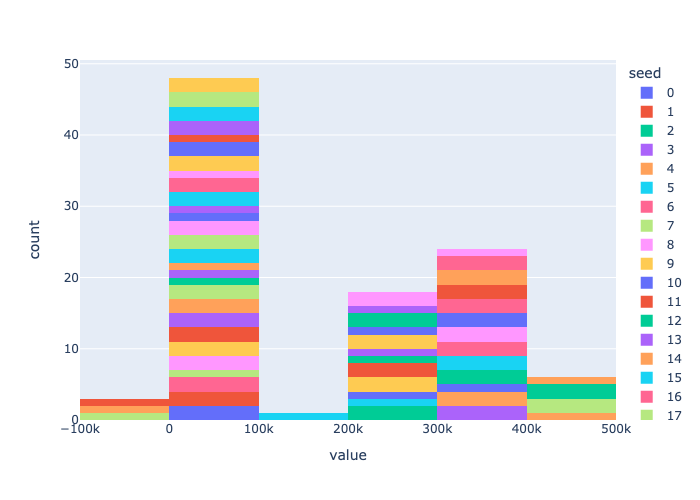
\includegraphics[width=\columnwidth]{assets/end-of-second-year-distribution.png}
\caption{A chart showing the balance over for 50 experiments (current OpenTTDLab )}
\label{fig:first-year}
\end{figure}

\begin{figure}[h]
\centering
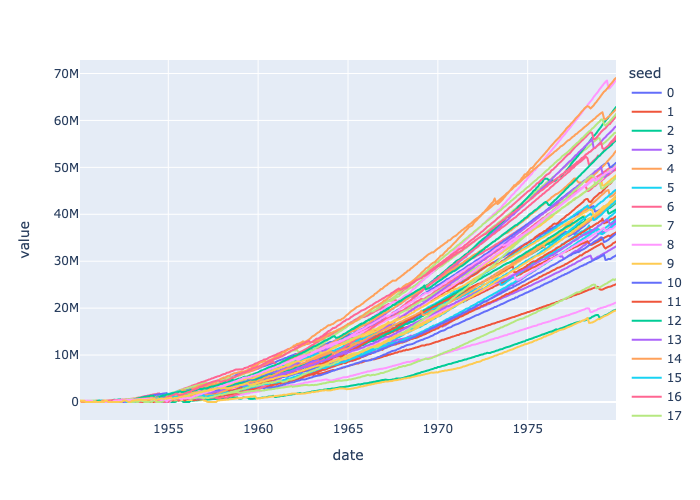
\includegraphics[width=\columnwidth]{assets/value-over-time-2.png}
\caption{A chart showing the balance over for 50 experiments (current OpenTTDLab )}
\label{fig:value-over-time}
\end{figure}

\begin{figure}[h]
\centering
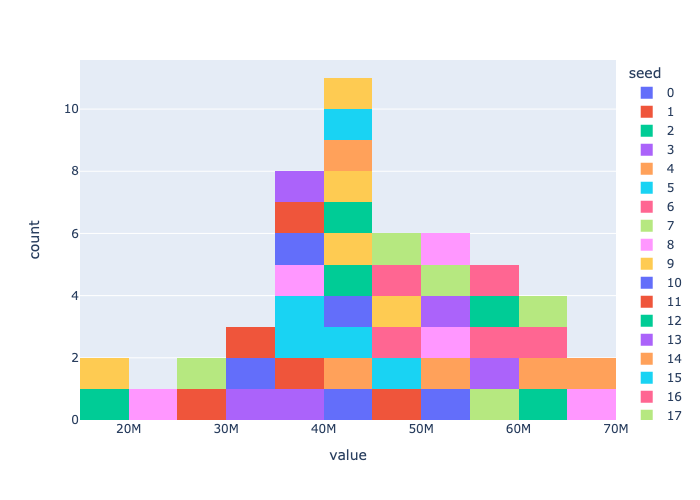
\includegraphics[width=\columnwidth]{assets/end-of-30th-year-distribution.png}
\caption{A chart showing the balance over for 50 experiments (current OpenTTDLab )}
\label{fig:first-year}
\end{figure}

\begin{figure}[h]
\centering
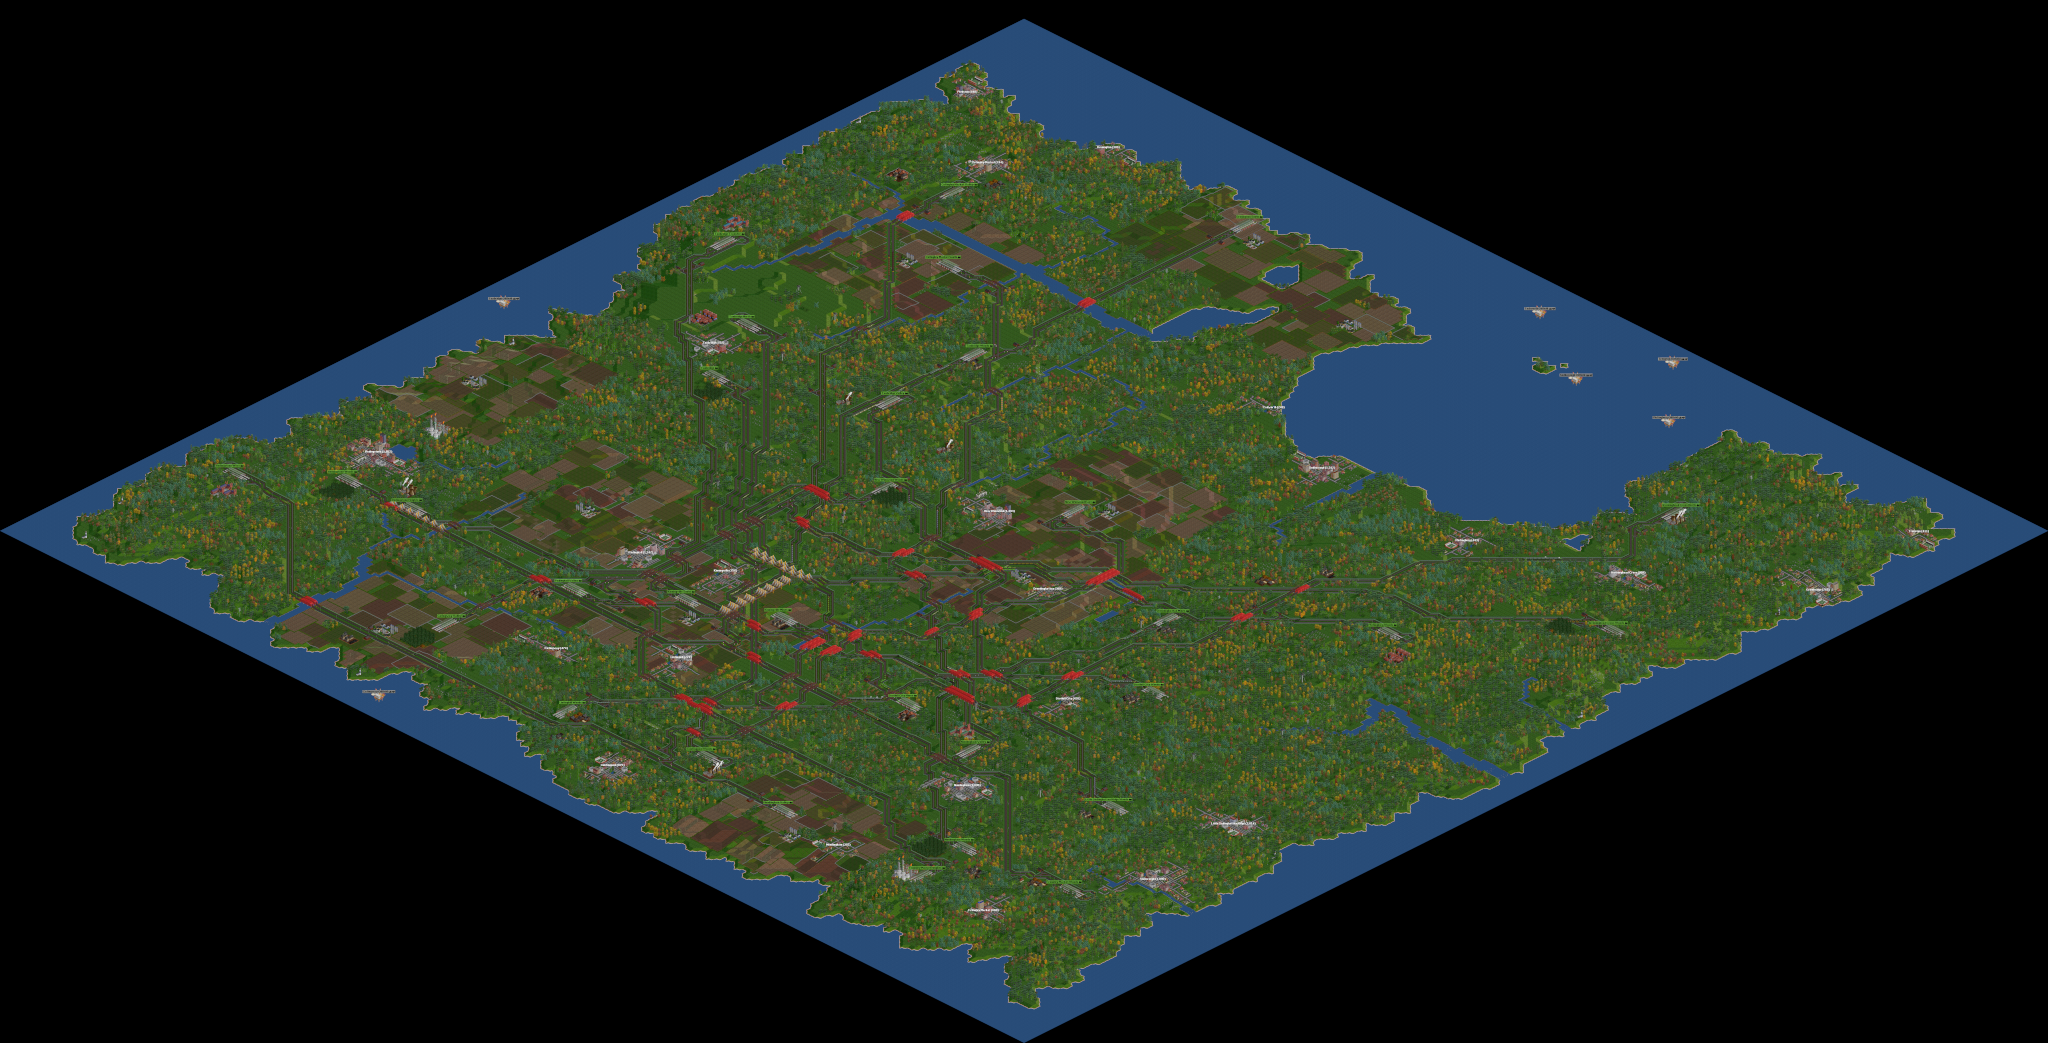
\includegraphics[width=\columnwidth]{assets/34_small.png}
\caption{Seed 34 - with the highest money at end}
\label{fig:openttd}
\end{figure}

\begin{figure}[h]
\centering
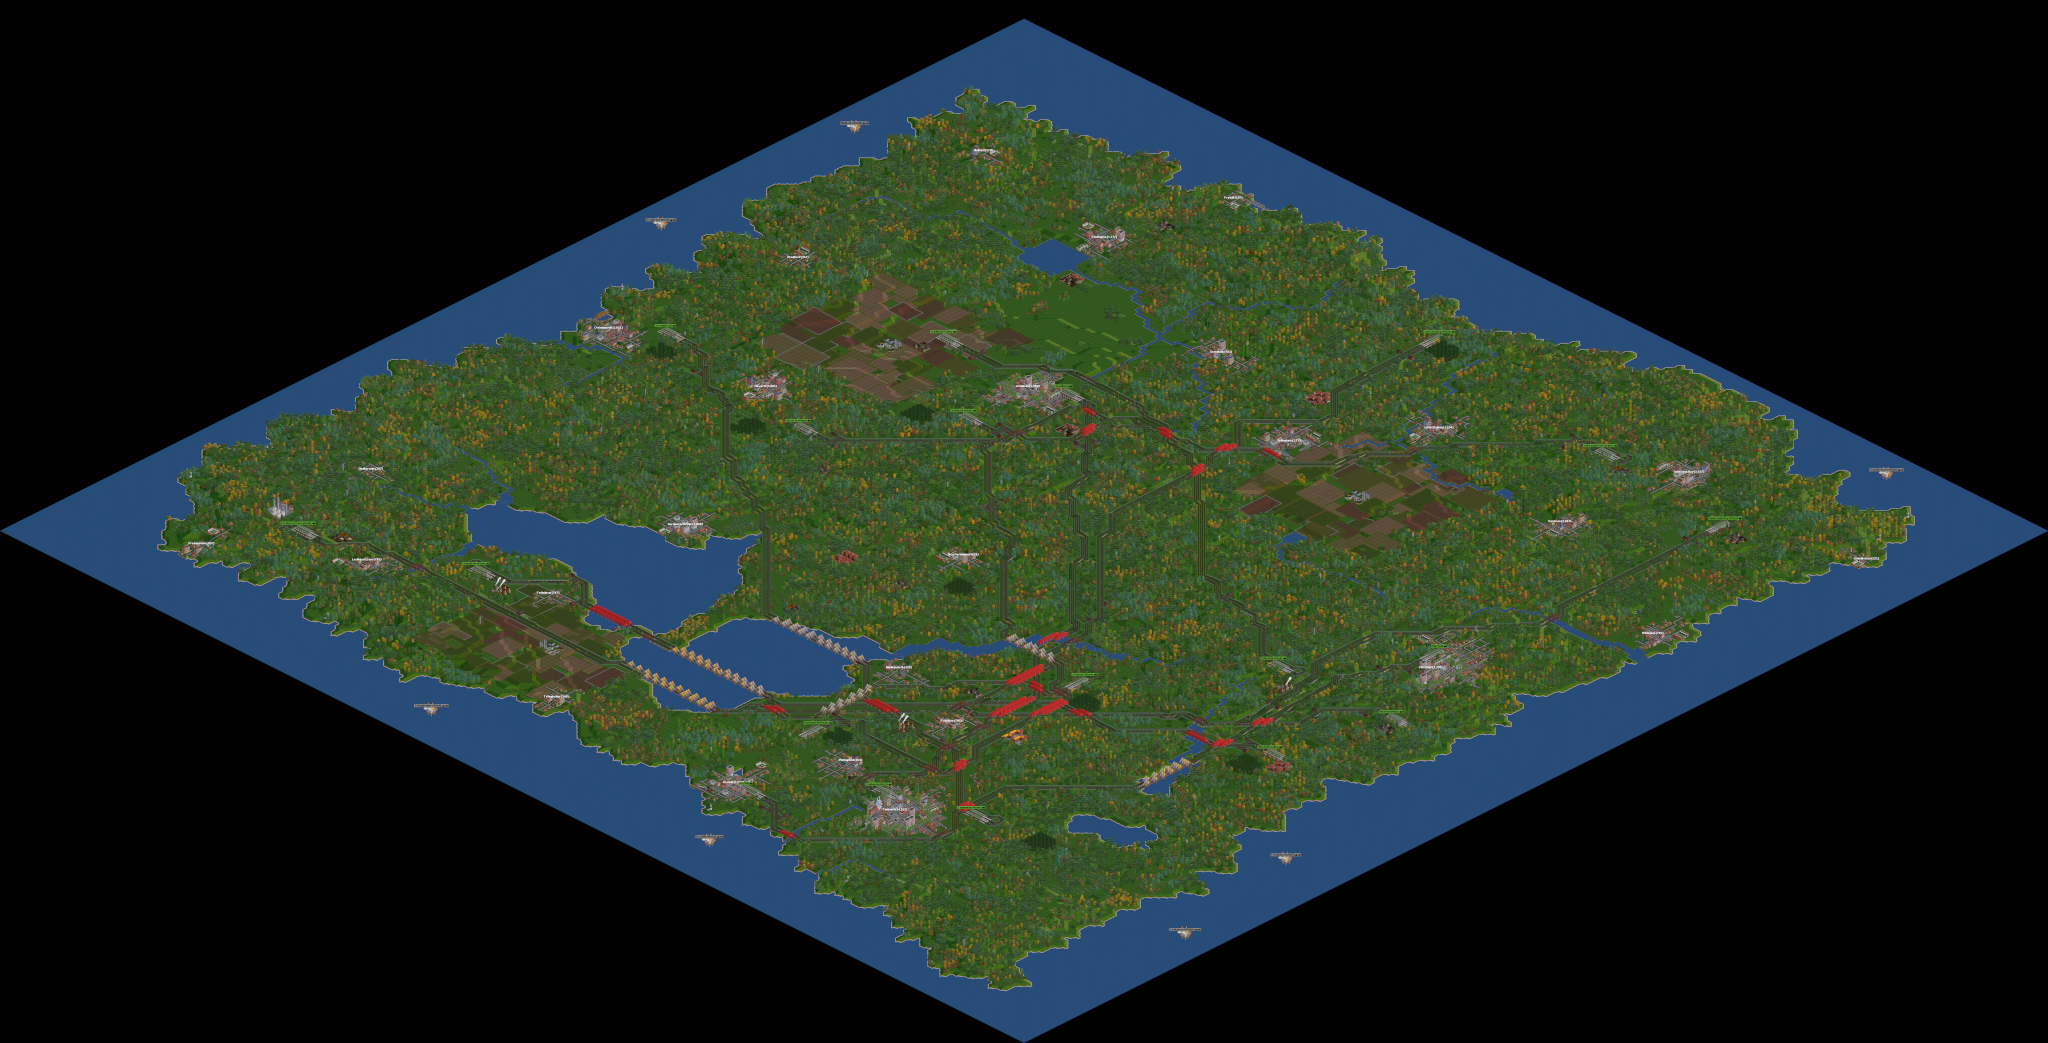
\includegraphics[width=\columnwidth]{assets/19_small.png}
\caption{Seed 19 - with the lowest money at end}
\label{fig:openttd}
\end{figure}

\begin{figure}[h]
\centering
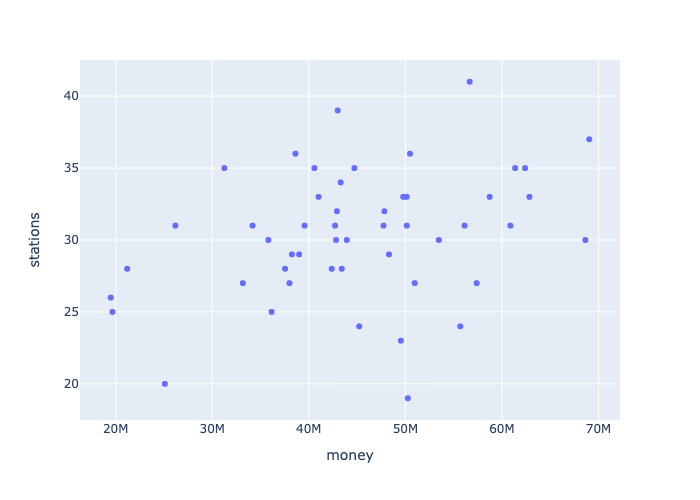
\includegraphics[width=\columnwidth]{assets/stations_vs_money.png}
\caption{Not much of a corrolation between stations and money!}
\label{fig:openttd}
\end{figure}

Bit of a "story" - starts off 300k. Then after a time there is a bi-modal distribution on money, then all the companies have have money in a normal-ish distribution.

Looks like the one with more stations/routes has more money? Can we corrolate stations with money?




------

\begin{figure}[h]
\centering
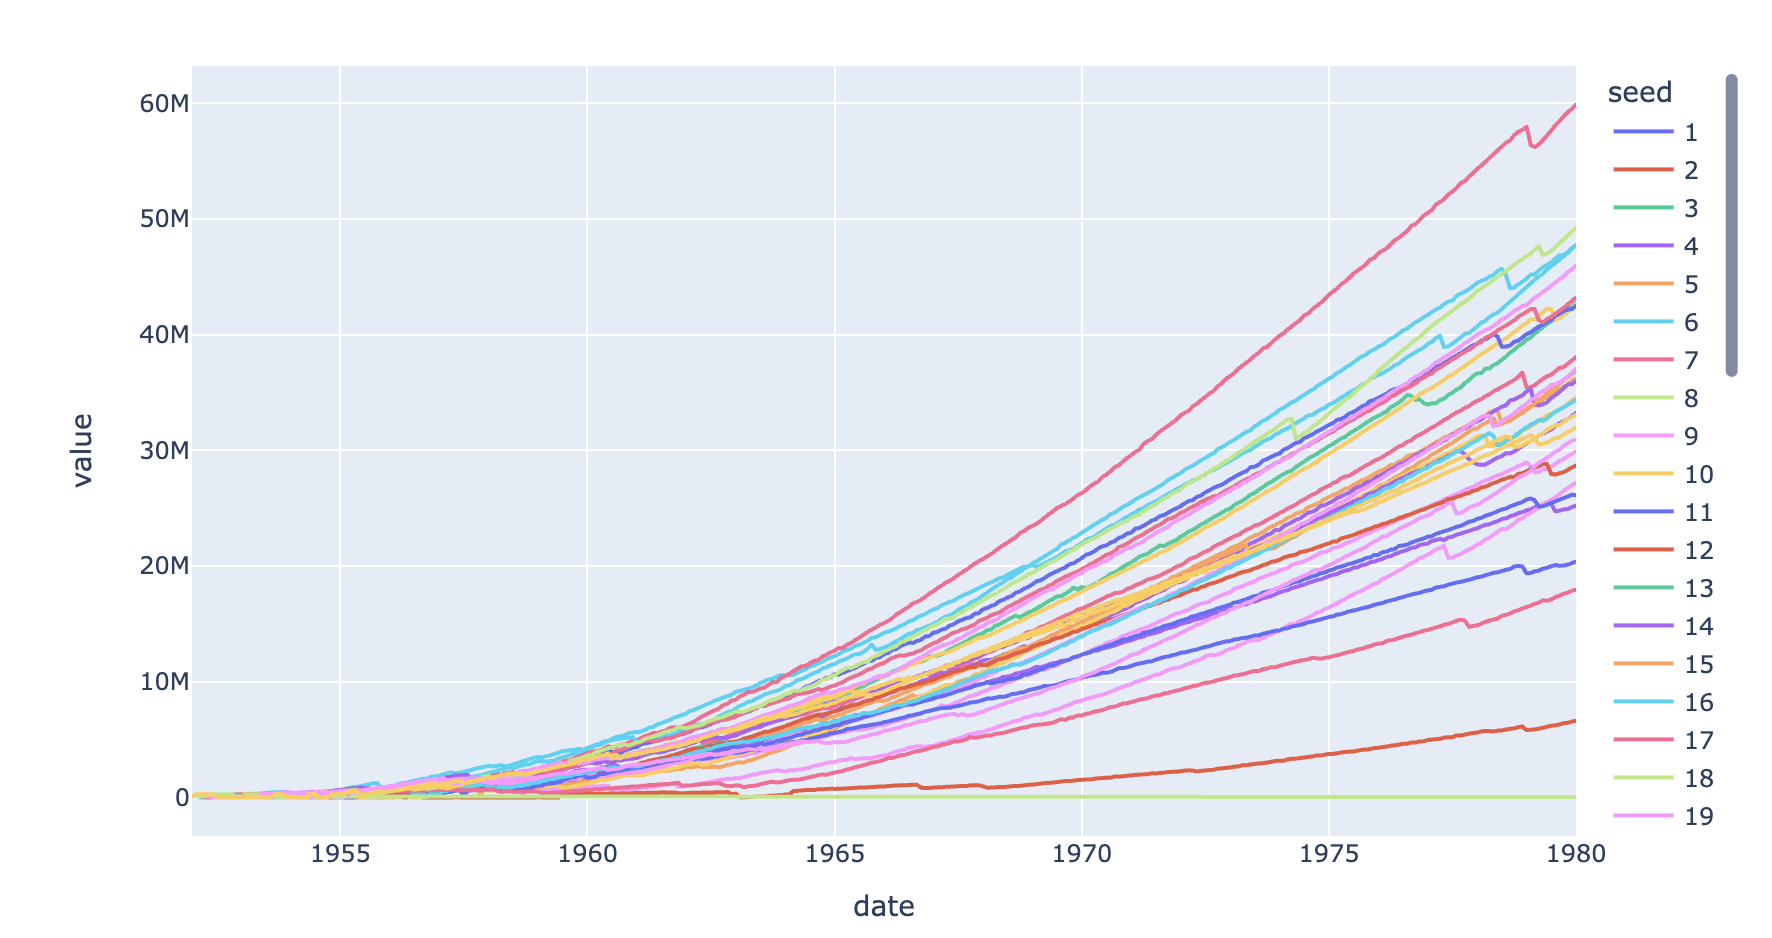
\includegraphics[width=\columnwidth]{assets/value-over-time.png}
\caption{A chart showing the balance over for 50 experiments (old version of OpenTTDLab - can't reproduce! Suspect because now AIs are started immediately, and so the random numbers are different? Will check on older OpenTTDLab)}
\label{fig:value-over-time}
\end{figure}







\chapter{Conclusion}

\begin{itemize}
\begin{item}
Maybe mention the link between this and testing here? Or should it be earlier?
\end{item}
\end{itemize}

The framework presented here allows experiments to be conducted with OpenTTD in a manner that is repeatable and reproducible. Reproducibility is up to the author's descriptions of the artefacts they created - they must be sufficient to recreate the artefacts, and so beyond the scope of the framework here. However, it should at least ease issues due to creating a similar enough experimental setup.

The exception are the version of the AI used - these do not appear to be versioned. However, potentially it could report on some sort of hash of the code of the AI.

Loads of further work... reproducible: version stuff, action, file format to save for example? Parallelise, easier optimisation

\chapter{Notes}

History

\begin{itemize}

\begin{item}
\cite{jackson1959learning} first business simulation game, US Air force MONOPOLOGS pretend to be inventory managers
\end{item}

\begin{item}
\cite{meijer2009organisation} - Studying supply chains using gaming simulation
\end{item}

\begin{item}
\cite{mayer2009gaming} - Defines simulation game as a game "experi(m)ent(i)al, rule-based, interactive environments, where players learn by taking actions and by experiencing their effects through feedback mechanisms that are deliberately built into and around the game"
\end{item}

\begin{item}
\cite{raghothama2013review} war gaming roots, policy analysis, business simulation games, studies on human cognition and behavior, training and pedagogical tools

Main point: simulation games particular suited for transportation research in general, and supply chain specifically because it's an emergent property

Some features of OpenTTD realistic, but this isn't exactly justified

Simutrans mentioned - described as not being realistic at all, but is extensible so could be

But similuation games not used for transportation

Gives lots of examples of simulation games used for research, but also mentions "Little attention has been paid to the validation of these simulation games."

(But: by and large here we're not concerning ourselves with validation)
\end{item}

\begin{item}
Basically have a list of a good range of how similuation games have been used.
\end{item}

\begin{item}
\cite{alderliesten2019maintrain} The simulation game itself used to try to get sympathy/understanding from passengers about delays
\end{item}

\begin{item}
\cite{cimellaro2016computational} - it lists OpenTTD alongside "real" simulators of cities in discussion for disaster reliance, with no particular mention that's it a game/for entertainment??
\end{item}

Repeatability


\begin{itemize}
\begin{item}
\cite{dalle2012reproducibility} in simulation in particular "many published works based on simulation still fail to meet the minimum conditions to ensure reproducibility" (and in my opinion the OpenTTD ones are no exception). And it gives some "levels" L1, L2, L3, L4 on how to judge "how" reproducbiel simulations are and highlights specific desirable details about simulations. I can probably judge some existing research using this, and compare to maybe output using my OpenTTDLab thing?

Hidden details that prevent reproducilibty (it cites another source for this)

I quite like this one! (TODO Check things that cite it especially)

"Goes beyond" reproducibility into traceability...

"– a simulator refers to a reusable simulation engine and its Application Programming Interface
(API); the engine is reusable for the simulation of many models and scenarios;" OpenTTDLab I think is the "missing" simulator??

"In simulation, not only the same sources of error
exist, but the system itself can be modeled incorrectly and be a source of error"

"Furthermore, as will be explained in greater details
in the next section, simulation has many applications that are not aimed toward producing science
and, therefore, do not necessarily require a reproducibility based on the source code availability."

"• manipulation errors: These errors result from the manual handling of some of the tasks in the simulation study work-flow."

OpenTTDLab I think addresses loads of the issues mentioned, in many of the ways it suggests.
\end{item}


\begin{item}
\cite{monks2019strengthening} - Checklist style "STRESS" guidelines. Strengthening the Reporting of Empirical Simulation Studies

It also has a review of lots of other guidelines for reproducible simulations

TODO: if going this way, reflect on the bits that OpenTTDLab does not do

"Agent-Based Simulation (ABS), Discrete-Event Simulation (DES) and System Dynamics (SD)." - er... OpenTTD is which of these??

"it is critical that author report the software version and build numbers" - this is for commercial software, but I would argue for Open Source as well
\end{item}

\begin{item}
Gass (1984) provides the earliest example of reporting guidelines for “computer based models”.
\end{item}
\end{itemize}

\end{itemize}


\bibliographystyle{plain}
\bibliography{mybibfile}


% You may delete everything from \appendix up to \end{document} if you don't need it.
\appendix

\chapter{First appendix}

\section{First section}

Any appendices, including any required ethics information, should be included
after the references.

Markers do not have to consider appendices. Make sure that your contributions
are made clear in the main body of the dissertation (within the page limit).


\end{document}
